
\documentclass[letterpaper,hide notes,xcolor={table,svgnames},pdftex]{beamer}
\def\showexamples{t}


%\usepackage[svgnames]{xcolor}

%% Demo talk
%\documentclass[letterpaper,notes=show]{beamer}

\usecolortheme{crane}
\setbeamertemplate{navigation symbols}{}

\usetheme{MyPittsburgh}
%\usetheme{Frankfurt}

%\usepackage{tipa}

\usepackage{hyperref}
\usepackage{graphicx,xspace}
\usepackage[normalem]{ulem}

\newcommand\SF[1]{$\bigstar$\footnote{SF: #1}}



\newcounter{tmpnumSlide}
\newcounter{tmpnumNote}

% old question code
%\newcommand\question[1]{{$\bigstar$ \small \onlySlide{2}{#1}}}
% \newcommand\nquestion[1]{\ifdefined \presentationonly \textcircled{?} \fi \note{\par{\Large \textbf{?}} #1}}
% \newcommand\nanswer[1]{\note{\par{\Large \textbf{A}} #1}}


 \newcommand\mnote[1]{%
   \addtocounter{tmpnumSlide}{1}
   \ifdefined\showcues {~\tiny\fbox{\arabic{tmpnumSlide}}}\fi
   \note{\setlength{\parskip}{1ex}\addtocounter{tmpnumNote}{1}\textbf{\Large \arabic{tmpnumNote}:} {#1\par}}}

\newcommand\mmnote[1]{\note{\setlength{\parskip}{1ex}#1\par}}

%\newcommand\mnote[2][]{\ifdefined\handoutwithnotes {~\tiny\fbox{#1}}\fi
% \note{\setlength{\parskip}{1ex}\textbf{\Large #1:} #2\par}}

%\newcommand\mnote[2][]{{\tiny\fbox{#1}} \note{\setlength{\parskip}{1ex}\textbf{\Large #1:} #2\par}}

\newcommand\mquestion[2]{{~\color{red}\fbox{?}}\note{\setlength{\parskip}{1ex}\par{\Large \textbf{?}} #1} \note{\setlength{\parskip}{1ex}\par{\Large \textbf{A}} #2\par}\ifdefined \presentationonly \pause \fi}

\newcommand\blackboard[1]{%
\ifdefined   \showblackboard
  {#1}
  \else {\begin{center} \fbox{\colorbox{blue!30}{%
         \begin{minipage}{.95\linewidth}%
           \hspace{\stretch{1}} Some space intentionally left blank; done at the blackboard.%
         \end{minipage}}}\end{center}}%
         \fi%
}



%\newcommand\q{\tikz \node[thick,color=black,shape=circle]{?};}
%\newcommand\q{\ifdefined \presentationonly \textcircled{?} \fi}

\usepackage{listings}
\lstset{%
  keywordstyle=\bfseries,
  aboveskip=15pt,
  belowskip=15pt,
  captionpos=b,
  identifierstyle=\ttfamily,
  escapeinside={(*@}{@*)},
  stringstyle=\ttfamiliy,
  frame=lines,
  numbers=left, basicstyle=\scriptsize, numberstyle=\tiny, stepnumber=0, numbersep=2pt}

\usepackage{siunitx}
\newcommand\sius[1]{\num[group-separator = {,}]{#1}\si{\micro\second}}
\newcommand\sims[1]{\num[group-separator = {,}]{#1}\si{\milli\second}}
\newcommand\sins[1]{\num[group-separator = {,}]{#1}\si{\nano\second}}
\sisetup{group-separator = {,}, group-digits = true}

%% -------------------- tikz --------------------
\usepackage{tikz}
\usetikzlibrary{positioning}
\usetikzlibrary{arrows,backgrounds,automata,decorations.shapes,decorations.pathmorphing,decorations.markings,decorations.text}

\tikzstyle{place}=[circle,draw=blue!50,fill=blue!20,thick, inner sep=0pt,minimum size=6mm]
\tikzstyle{transition}=[rectangle,draw=black!50,fill=black!20,thick, inner sep=0pt,minimum size=4mm]

\tikzstyle{block}=[rectangle,draw=black, thick, inner sep=5pt]
\tikzstyle{bullet}=[circle,draw=black, fill=black, thin, inner sep=2pt]

\tikzstyle{pre}=[<-,shorten <=1pt,>=stealth',semithick]
\tikzstyle{post}=[->,shorten >=1pt,>=stealth',semithick]
\tikzstyle{bi}=[<->,shorten >=1pt,shorten <=1pt, >=stealth',semithick]

\tikzstyle{mut}=[-,>=stealth',semithick]

\tikzstyle{treereset}=[dashed,->, shorten >=1pt,>=stealth',thin]

\usepackage{ifmtarg}
\usepackage{xifthen}
\makeatletter
% new counter to now which frame it is within the sequence
\newcounter{multiframecounter}
% initialize buffer for previously used frame title
\gdef\lastframetitle{\textit{undefined}}
% new environment for a multi-frame
\newenvironment{multiframe}[1][]{%
\ifthenelse{\isempty{#1}}{%
% if no frame title was set via optional parameter,
% only increase sequence counter by 1
\addtocounter{multiframecounter}{1}%
}{%
% new frame title has been provided, thus
% reset sequence counter to 1 and buffer frame title for later use
\setcounter{multiframecounter}{1}%
\gdef\lastframetitle{#1}%
}%
% start conventional frame environment and
% automatically set frame title followed by sequence counter
\begin{frame}%
\frametitle{\lastframetitle~{\normalfont(\arabic{multiframecounter})}}%
}{%
\end{frame}%
}
\makeatother

\makeatletter
\newdimen\tu@tmpa%
\newdimen\ydiffl%
\newdimen\xdiffl%
\newcommand\ydiff[2]{%
    \coordinate (tmpnamea) at (#1);%
    \coordinate (tmpnameb) at (#2);%
    \pgfextracty{\tu@tmpa}{\pgfpointanchor{tmpnamea}{center}}%
    \pgfextracty{\ydiffl}{\pgfpointanchor{tmpnameb}{center}}%
    \advance\ydiffl by -\tu@tmpa%
}
\newcommand\xdiff[2]{%
    \coordinate (tmpnamea) at (#1);%
    \coordinate (tmpnameb) at (#2);%
    \pgfextractx{\tu@tmpa}{\pgfpointanchor{tmpnamea}{center}}%
    \pgfextractx{\xdiffl}{\pgfpointanchor{tmpnameb}{center}}%
    \advance\xdiffl by -\tu@tmpa%
}
\makeatother
\newcommand{\copyrightbox}[3][r]{%
\begin{tikzpicture}%
\node[inner sep=0pt,minimum size=2em](ciimage){#2};
\usefont{OT1}{phv}{n}{n}\fontsize{4}{4}\selectfont
\ydiff{ciimage.south}{ciimage.north}
\xdiff{ciimage.west}{ciimage.east}
\ifthenelse{\equal{#1}{r}}{%
\node[inner sep=0pt,right=1ex of ciimage.south east,anchor=north west,rotate=90]%
{\raggedleft\color{black!50}\parbox{\the\ydiffl}{\raggedright{}#3}};%
}{%
\ifthenelse{\equal{#1}{l}}{%
\node[inner sep=0pt,right=1ex of ciimage.south west,anchor=south west,rotate=90]%
{\raggedleft\color{black!50}\parbox{\the\ydiffl}{\raggedright{}#3}};%
}{%
\node[inner sep=0pt,below=1ex of ciimage.south west,anchor=north west]%
{\raggedleft\color{black!50}\parbox{\the\xdiffl}{\raggedright{}#3}};%
}
}
\end{tikzpicture}
}


%% --------------------

%\usepackage[excludeor]{everyhook}
%\PushPreHook{par}{\setbox0=\lastbox\llap{MUH}}\box0}

%\vspace*{\stretch{1}

%\setbox0=\lastbox \llap{\textbullet\enskip}\box0}

\setlength{\parskip}{\fill}

\newcommand\noskips{\setlength{\parskip}{1ex}}
\newcommand\doskips{\setlength{\parskip}{\fill}}

\newcommand\xx{\par\vspace*{\stretch{1}}\par}
\newcommand\xxs{\par\vspace*{2ex}\par}
\newcommand\tuple[1]{\langle #1 \rangle}
\newcommand\code[1]{{\sf \footnotesize #1}}
\newcommand\ex[1]{\uline{Example:} \ifdefined \presentationonly \pause \fi
  \ifdefined\showexamples#1\xspace\else{\uline{\hspace*{2cm}}}\fi}

\newcommand\ceil[1]{\lceil #1 \rceil}


\AtBeginSection[]
{
   \begin{frame}
       \frametitle{Outline}
       \tableofcontents[currentsection]
   \end{frame}
}



\pgfdeclarelayer{edgelayer}
\pgfdeclarelayer{nodelayer}
\pgfsetlayers{edgelayer,nodelayer,main}

\tikzstyle{none}=[inner sep=0pt]
\tikzstyle{rn}=[circle,fill=Red,draw=Black,line width=0.8 pt]
\tikzstyle{gn}=[circle,fill=Lime,draw=Black,line width=0.8 pt]
\tikzstyle{yn}=[circle,fill=Yellow,draw=Black,line width=0.8 pt]
\tikzstyle{empty}=[circle,fill=White,draw=Black]
\tikzstyle{bw} = [rectangle, draw, fill=blue!20, 
    text width=4em, text centered, rounded corners, minimum height=2em]
    
    \newcommand{\CcNote}[1]{% longname
	This work is licensed under the \textit{Creative Commons #1 3.0 License}.%
}
\newcommand{\CcImageBy}[1]{%
	\includegraphics[scale=#1]{creative_commons/cc_by_30.pdf}%
}
\newcommand{\CcImageSa}[1]{%
	\includegraphics[scale=#1]{creative_commons/cc_sa_30.pdf}%
}
\newcommand{\CcImageNc}[1]{%
	\includegraphics[scale=#1]{creative_commons/cc_nc_30.pdf}%
}
\newcommand{\CcGroupBySa}[2]{% zoom, gap
	\CcImageBy{#1}\hspace*{#2}\CcImageNc{#1}\hspace*{#2}\CcImageSa{#1}%
}
\newcommand{\CcLongnameByNcSa}{Attribution-NonCommercial-ShareAlike}

\newenvironment{changemargin}[1]{% 
  \begin{list}{}{% 
    \setlength{\topsep}{0pt}% 
    \setlength{\leftmargin}{#1}% 
    \setlength{\rightmargin}{1em}
    \setlength{\listparindent}{\parindent}% 
    \setlength{\itemindent}{\parindent}% 
    \setlength{\parsep}{\parskip}% 
  }% 
  \item[]}{\end{list}} 



\usepackage{alltt}

\title{Lecture 15 --- Testing: Intro \& JUnit}

\author{Jeff Zarnett \& Patrick Lam \\ \small \texttt{jzarnett@uwaterloo.ca} \& \texttt{p.lam@ece.uwaterloo.ca}}
\institute{Department of Electrical and Computer Engineering \\[-1ex]
  University of Waterloo}
\date{\today}

\begin{document}

\begin{frame}
  \titlepage

\end{frame}

\begin{frame}
\frametitle{Software Testing}
\begin{changemargin}{1cm}
\alert{Testing} attempts to verify the functionality of software.

It is somewhat like testing physical systems.

But software can fail in many bizarre ways.

Most problems: design problems, not manufacturing problems.

Software does not corrode; so problems were always there.

\mnote{4th year course, ECE 453}
\end{changemargin}
\end{frame}


\begin{frame}
\frametitle{Software Testing}
\begin{changemargin}{1cm}
Software bugs are a fact of life. Not because programmers are careless; because software's complex.

Human ability to deal with complexity is limited.

We can have problems of design or implementation.

Programs are dynamic: a change can have side effects.

A test that previously passed might now fail.

\end{changemargin}
\end{frame}

\begin{frame}
\frametitle{Software Testing}
\begin{changemargin}{1cm}
It will never be possible to test software completely.

We cannot guarantee a bug-free program.

But testing makes our software better.

\end{changemargin}
\end{frame}


\begin{frame}
\frametitle{Software Testing}
\begin{changemargin}{1cm}
NIST says that in 2002, software bugs cost the US economy: \$59.5 Billion.

They estimate $1/3$ could be saved with better testing practice.

The earlier a bug is found, the cheaper it is to fix.

\end{changemargin}
\end{frame}

\begin{frame}
\frametitle{Software Testing}
\begin{changemargin}{1cm}

When testing, you'll run \alert{test suites} consisting of \alert{test
  cases}.

A \emph{test case} contains:
\begin{itemize}
\item what you feed to software; and
\item what the software should output in response.  
\end{itemize} 

You can organize the collection of test cases you need to write
according to a \emph{test plan}.

\end{changemargin}
\end{frame}

\begin{frame}
\frametitle{Knowing the Answer}
\begin{changemargin}{1cm}
We have to know what is the correct output, independent of the actual output of the software

Dangerous if we don't know that answer.

Tests are often written after implementation and just use the current output as correct.

Imagine if the function returns $2 + 2 = 5$ and a programmer wrote a test that expects the answer $5$!

\end{changemargin}
\end{frame}


\begin{frame}
\frametitle{Testing vs. Correctness}
\begin{changemargin}{1cm}

Common view: testing is only for finding defects.

Recent research allows proving correctness with testing.

\end{changemargin}
\end{frame}

\begin{frame}
\frametitle{Levels of Testing}
\begin{changemargin}{1cm}

\subsection*{Levels of Testing}
Testing is often performed at several different levels:
\begin{itemize}
\item Smoke tests \mnote{are the most basic of checks.}
\item Unit tests \mnote{are low-level tests which verify the functionality of
a single class (or unit) at a time.}
\item Integration tests \mnote{combine more than one unit and verify the
functionality of the interfaces between components.}
\item Stress tests \mnote{run to see how components or systems behave when under pressure.}
\item System tests \mnote{run on the entire system, after it has been
integrated, and verify that everything works right.}
\end{itemize}


\end{changemargin}
\end{frame}

\begin{frame}
\frametitle{Smoke Testing}
\begin{changemargin}{1cm}


\begin{center}
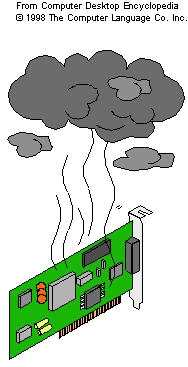
\includegraphics[width=0.3\textwidth]{images/smoke-test.png}
\end{center}

\mnote{The term comes from electrical engineering... if you turn on your circuit and smoke comes out, something is catastrophically wrong. Sometimes we do this in software as well; a minimal set of tests to be sure that the system starts up and runs without anything going disastrously wrong. However, smoke tests do not ensure anything about the program other than it turns on without smoke streaming out.}

\mnote{Minimal tests might be: server boots up, client launches, users can log in.}

\end{changemargin}
\end{frame}


\begin{frame}
\frametitle{Unit Testing}

\begin{changemargin}{1cm}

\Large
Units: small parts of a software system (methods, classes, sets of classes).\\[1em]

Two Key Ideas:
\begin{enumerate}
\item Test units independently.
\item Specify desired behaviour using tests.
\end{enumerate}

\end{changemargin}

\end{frame}

\begin{frame}
\frametitle{Properties of Unit Tests}
\begin{changemargin}{1cm}
\begin{itemize}
	\item Focus on the unit being tested \mnote{don't depend on a database, network, or other external resources}
	\item Easy to run \mnote{(e.g. by setting them up as JUnit tests): they must incur no setup costs to run nor require user input; they can therefore serve as regression tests;
}
	\item Easy to write \mnote{(a few minutes per test) and focus on one aspect of behaviour; they should tell you something about the unit.}
\end{itemize}

Some advice on Unit Testing:

\begin{itemize}
\item specify and document the requirements of the unit.
\item test behaviour, not state; use mock objects to verify behaviour.
\item Test-Driven Development: write tests before the code.
\end{itemize}

\end{changemargin}
\end{frame}


\begin{frame}
\frametitle{About JUnit}

\begin{changemargin}{1cm}
\large

Most popular unit testing framework for Java.\\[1em]

Tests depend on the notion of \alert{assertions}.

\end{changemargin}

\end{frame}

\begin{frame}
\frametitle{Assertions}
\begin{changemargin}{1cm}

An assertion is a statement about the world.

In code, logical expression that should always be true.

If not, throw \texttt{AssertionError}.

This usually stops the program. \mnote{Assertions are usually not left in the code that is released}

\end{changemargin}

\end{frame}



\begin{frame}
\frametitle{Objective: Unit Tests}

\begin{changemargin}{1.5cm}

Learn how to write simple JUnit 
tests for Java code.\\[1em]

Use {\tt assertTrue} or {\tt
  assertEquals} to verify test results.
\end{changemargin}

\end{frame}

\begin{frame}
\frametitle{JUnit Test Organization}

\large
\begin{changemargin}{1cm}
JUnit tests belong to test classes.\\[1em]

A test:
\begin{itemize}
\item is labelled {\tt @org.junit.Test};
\item is a method with no parameters;
\item makes calls to the class under test;
\item verifies that the class is doing the right thing using assertions.
\end{itemize}

\end{changemargin}
\end{frame}

\begin{frame}
\frametitle{Using JUnit Tests}

\begin{changemargin}{1cm}

After writing the tests:
\begin{enumerate}
\item press a button in your IDE;
\item it will run the tests automatically for you.
\end{enumerate}
\end{changemargin}

If the tests fail:

\begin{center}
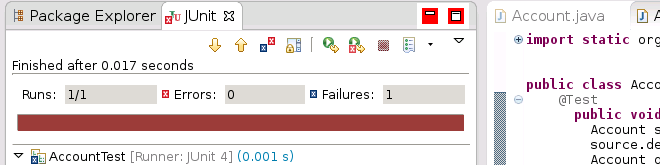
\includegraphics[width=0.6\textwidth]{images/fail.png}
\end{center}

If the tests pass:

\begin{center}
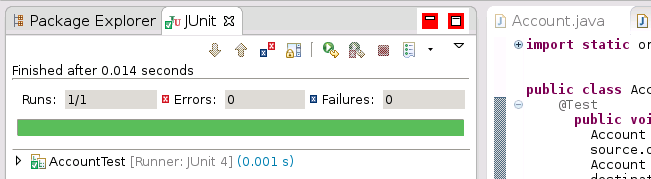
\includegraphics[width=0.6\textwidth]{images/pass.png}
\end{center}

\end{frame}

\begin{frame}
\frametitle{Why Unit Tests?}

\begin{changemargin}{1cm}
Biggest benefit of unit tests:
\begin{itemize}
\item they can run automatically.
\end{itemize}
You'll never run tests that are annoying to run.

\end{changemargin}
\end{frame}


\begin{frame}[fragile]
\frametitle{Account Example}

\begin{lstlisting}[language={Java},basicstyle=\scriptsize]
public class Account
{
  private float balance;
  public void deposit (float amount) { balance += amount; }

  public void withdraw (float amount) { balance -= amount; }

  public void transferFunds(Account destination, float amount) {
  }

  public float getBalance() { return balance; }
}
\end{lstlisting}

\end{frame}

\begin{frame}[fragile]
\frametitle{JUnit Test for Account}
Let's write a unit test for this class:

\begin{lstlisting}[language={Java},basicstyle=\scriptsize]
import static org.junit.Assert.*;
import org.junit.Test;

public class AccountTest {
  @Test
  public void transferFunds() {
    Account source = new Account();
    source.deposit(200.00f);
    Account destination = new Account();
    destination.deposit(150.00f);

    source.transferFunds(destination, 100.00f);
    assertEquals(``destination balance``, 250.00f, 
                 destination.getBalance(), 0.01);
    assertEquals(``source balance``, 100.00f, 
                 source.getBalance(), 0.01);
  }
}
\end{lstlisting}
\end{frame}

\begin{frame}[fragile]
\frametitle{Test Results}

\begin{changemargin}{1.5cm}
If we run this test, we'd get a red bar; {\tt transferFunds} doesn't
do anything. Adding this code:

\begin{lstlisting}[language={Java},basicstyle=\scriptsize]
public void transferFunds(Account destination, float amount) {
    destination.deposit(amount);
    withdraw(amount);
}
\end{lstlisting}
makes the bar green, since the test now passes.
\end{changemargin}
\end{frame}

\begin{frame}[fragile]
\frametitle{JUnit Test Fixtures}

\begin{changemargin}{1cm}
Tests often share objects.\\[1em]

Repeatedly allocating these objects is terrible.\\[1em]

Solution: test fixtures.

\begin{lstlisting}[language={Java},basicstyle=\scriptsize]
public class AccountTest {
  private Account account1;

  // runs before any tests
  @Before public void setUp() {
    account1 = new Account(); 
    account1.deposit(200.00f);
  }
}
\end{lstlisting}

Use {\tt @After} to free resources afterwards.\\[1em]

\alert{Caveat:} Don't rely on object state between tests: JUnit may shuffle order.
\end{changemargin}
\end{frame}

\begin{frame}[fragile]
\frametitle{Expected Exceptions}

\begin{changemargin}{1cm}
How do you test error-checking code?\\[1em]

\pause
It should throw exceptions!\\[1em]

Make the test case expect an exception.\\[1em]
From the JUnit cookbook:
\end{changemargin}

\begin{lstlisting}
@Test(expected=IndexOutOfBoundsException.class) 
public void empty() { 
    new ArrayList<Object>().get(0); 
}
\end{lstlisting}

\end{frame}

\begin{frame}
\frametitle{JUnit 4 versus JUnit 3}

\begin{changemargin}{1.5cm}
So far, we saw the (better) JUnit 4 syntax.\\[1em]

Android uses JUnit 3 syntax. Key differences:

\begin{itemize}
\item test classes must extend {\tt TestCase};
\item test names must start with {\tt test};
\item fixture setup method must be called {\tt setUp()};
\item fixture teardown method must be called {\tt tearDown()};
\item testing exceptions is harder.
\end{itemize}

\end{changemargin}
\end{frame}


\begin{frame}[fragile]
\frametitle{Useful Concept (not just for Testing)}

\begin{changemargin}{1.5cm}

Imagine a JUnit test for a piece of code that is used for data retrieval. 

You have a set of student IDs and student names. 

You might have two \texttt{Array} objects, defined like this:

{\tiny
\begin{verbatim}
private ArrayList<String> studentIDs = {''20000000'', ''20000001'', ''20000002''};
private ArrayList<String> studentNames = {''John Doe'', ''Jane Doe'', ''Max Mustermann''};
\end{verbatim}
}


\end{changemargin}
\end{frame}

\begin{frame}
\frametitle{Useful Concept (not just for Testing)}
\begin{changemargin}{1.5cm}

Check: index in the array of Student IDs is the same as the array of Student Names and that the two arrays line up. 

Call the function \texttt{getName(studentIDs[i])}.

Check with an assertion statement that the name returned matches \texttt{studentNames[i]}. 

Can we have a relation between the student IDs and names without \texttt{i}?


\end{changemargin}
\end{frame}

\begin{frame}[fragile]
\frametitle{``Key'' Idea}
\begin{changemargin}{1.5cm}

A \alert{Key-Value Pair}. 

Key on the left; value on the right.


\begin{verbatim}
(''20000000'', ''John Doe'')
(''20000001'', ''Jane Doe'')
(''20000002'', ''Max Mustermann'')
\end{verbatim}

\end{changemargin}
\end{frame}


\begin{frame}
\frametitle{HashMap}
\begin{changemargin}{1.5cm}

The Java data structure to represent this is a \texttt{HashMap}.

A \texttt{HashMap} holds a set of keys and values.

Keys must be unique. A key corresponds to exactly 1 value.


\end{changemargin}
\end{frame}


\begin{frame}
\frametitle{HashMap vs. List}
\begin{changemargin}{1.5cm}

A list definition has a type: \texttt{ArrayList<String>}. 

A \texttt{HashMap} has two types:\\
\quad the type for the Key and the type for the Value. 

Example: \texttt{HashMap<String, Money>}. 

The types of the key and value can be anything, e.g., \texttt{Student} and \texttt{Address}.



\end{changemargin}
\end{frame}


\begin{frame}
\frametitle{HashMap vs. List}
\begin{changemargin}{1.5cm}

An \texttt{List} of type \texttt{T} is effectively a \texttt{HashMap<int, T>}. 

Give in an integer (0) and get a value (object of type \texttt{T}). 

The methods used have different names and signatures. \\
\quad But they are functionally the same. 

Their internal representations may be different.


\end{changemargin}
\end{frame}


\begin{frame}
\frametitle{How to Use a HashMap}
\begin{changemargin}{1.5cm}

To retrieve some data from the \texttt{HashMap}:

\texttt{get()} method with the key of the item you want: \texttt{get(''20000000'')} returns \texttt{''John Doe''}.


\end{changemargin}
\end{frame}


\begin{frame}
\frametitle{How to Use a HashMap}
\begin{changemargin}{1.5cm}


To add something to the \texttt{HashMap}, use the \texttt{put()} method, with the key and the value.

\texttt{put(``20000003'', ``Mel Mustermann'')} $\rightarrow$ new entry in the map. 

Already a value for the key? replaces the value: 

\texttt{put(''20000000'', ''Michael Doe'')} $\rightarrow$ \texttt{''Michael Doe''} replaces \texttt{''John Doe''} in the map.


\end{changemargin}
\end{frame}

\begin{frame}
\frametitle{How to Use a HashMap}
\begin{changemargin}{1.5cm}


To remove something from the map, use the \texttt{remove()} method with the key of the item to remove: 

\texttt{remove(''20000001'')} $\rightarrow$ remove the entry \texttt{(''20000001'', ''Jane Doe'')} from the map.

\end{changemargin}
\end{frame}


\begin{frame}
\frametitle{How to Use a HashMap}
\begin{changemargin}{1.5cm}

To get a list of all the keys: \texttt{keySet()}.

(There are other methods: \texttt{clear(), containsKey(), containsValue(), isEmpty(), size()}...)


\end{changemargin}
\end{frame}

\begin{frame}[fragile]
\frametitle{Testing with the HashMap}
\begin{changemargin}{1.5cm}

Test our \texttt{getName(String studentID)} function using a \texttt{HashMap} called \texttt{hm}.

{\small
\begin{verbatim}
for (String key : hm.keySet()) {
    assertEquals(``Student Name'', 
                      hm.get(key), getName(key));
}
\end{verbatim}
}

\end{changemargin}
\end{frame}

\end{document}
